\let\zendcenter\endcenter\RequirePackage[l2tabu,orthodox]{nag}\let\endcenter\zendcenter
\documentclass[xcolor=dvipsnames,compress]{beamer}
% \usetheme{DarkConsole}
% \usetheme{metropolis}

% Filter out annoying warnings
\usepackage{silence}
\WarningFilter{nag}{table with no}
\WarningFilter{nag}{figure with no}

\usetheme{bjeldbak}
\usepackage{nimbusmononarrow}

% \renewcommand*\familydefault{\ttdefault}
% \usepackage[T1]{fontenc}
\usepackage{fontspec}
\setmainfont[Mapping=tex-text]{Roboto Mono}
\let\sfdefault\rmdefault

\usepackage[l2tabu,orthodox]{nag}
\usepackage{ifthen}
\usepackage[linesnumbered]{algorithm2e}
\usepackage[lambda,landau,operators,probability,sets,logic,advantage,complexity,asymptotics,notions,mm,primitives,ff,adversary]{cryptocode}
\usepackage{listings}
\usepackage{multicol}
\usepackage{wasysym}
\usepackage{csquotes}
\usepackage{bm}

\usepackage{multirow}
\usepackage{booktabs}  %% tables
\usepackage{tikz,pgfplots}
\usetikzlibrary{shapes,arrows,positioning,automata,matrix,calc,decorations.pathreplacing,spy}
\tikzset{
	arrowthick/.style={shorten >=0.2cm,shorten <=0.2cm,-diamond,draw=black,thick},arrow/.style={shorten >=0.1cm,shorten <=0.1cm,-diamond,draw=black},
	mat/.style={draw=black,minimum width=1.5em,minimum height=1.5em},matblank/.style={minimum width=1.5em,minimum height=1.5em}
}
\newcommand{\tikzmark}[1]{\tikz[overlay,remember picture] \node (#1) {};}
\usepackage{multimedia}
\usepackage{mathtools}
\usepackage{colortbl}

\usepackage{tcolorbox}
\usepackage{hyperref}

% itemize bullet styling
\newcommand*{\upbullet}{:::}
\newcommand*{\itemi}{\item[\upbullet]}
\setbeamertemplate{itemize item}{\upbullet}
\setbeamertemplate{bibliography item}{\insertbiblabel}
\newcommand{\wideitems}{\setlength\itemsep{1em}}

% custom legend text
\pgfplotsset{
	legend image with text/.style={
		legend image code/.code={%
			\node[anchor=center] at (0.3cm,0cm) {#1};
		}
	},
}

% colours
\definecolor{DarkRoyalBlue}{HTML}{332288}
\definecolor{DarkBlue}{HTML}{6699CC}
\definecolor{LightBlue}{HTML}{88CCEE}
\definecolor{DarkGreen}{HTML}{117733}
\definecolor{DarkRed}{HTML}{661100}
\definecolor{LightRed}{HTML}{CC6677}
\definecolor{LightPink}{HTML}{AA4466}
\definecolor{DarkPink}{HTML}{882255}
\definecolor{LightRoyalBlue}{HTML}{AA4499}

\definecolor{DarkBrown}{HTML}{604c38}
\definecolor{DarkTeal}{HTML}{23373b}
\definecolor{LightBrown}{HTML}{EB811B}
\definecolor{LightGreen}{HTML}{14B03D}
\definecolor{metropoli}{HTML}{004d4d}
\definecolor{orangeu}{HTML}{ff5c33}

\definecolor{VapourCyan}{HTML}{27B3B6}
\definecolor{VapourMagenta}{HTML}{FF00FF}

\usepackage{soul}
\newcommand*{\cbox}[2]{%
    \fboxsep=1pt%
    \fcolorbox{#2}{#2}{#1}%
}
\newcommand{\hlwhite}[1]{{\cbox{#1}{white}}}
\newcommand{\hlcyan}[1]{{\cbox{#1}{VapourCyan!30}}}
\newcommand{\hlorangeu}[1]{{\cbox{#1}{orangeu!30}}}
\newcommand{\hlmagenta}[1]{{\cbox{#1}{VapourMagenta!20}}}
\newcommand{\hlblue}[1]{{\cbox{#1}{LightBlue!60}}}

% Set title to the center
% \setbeamertemplate{frametitle}[default][center]
\setbeamertemplate{frametitle}{\vspace*{-1cm}}
\newcolumntype{o}{>{\columncolor{orangeu!30}}c}
\newcolumntype{v}{>{\columncolor{VapourMagenta!20}}c}
\newcolumntype{w}{>{\columncolor{white}}c}
\newcolumntype{x}{>{\columncolor{VapourCyan!30}}c}
\newcolumntype{y}{>{\columncolor{LightBlue!60}}c}

% titling
\newcommand{\intertitle}[1]{\vspace{0.1cm}\textbf{:: \textsc{#1} ::}\vspace{0.1cm}}
\newcommand{\centertitle}[1]{\begin{center}\intertitle{#1}\end{center}}

% macros
%
% style
%
\newcommand{\heading}[1]{{\vspace{6pt}\noindent\sc{#1.}}}
% \renewcommand{\paragraph}[1]{\heading{#1}}
\newcommand{\ith}[1]{\ensuremath{#1^{\text{th}}}\xspace}

%
% games
%
\newcommand{\Gm}{\ensuremath{\mathrm{Game}}\xspace}
\newcommand{\A}{\ensuremath{\mathcal{A}}\xspace}
\newcommand{\D}{\ensuremath{\mathcal{D}}\xspace}
\newcommand{\F}{\ensuremath{\mathcal{F}}\xspace}
\newcommand{\K}{\ensuremath{\mathcal{K}}\xspace}
\newcommand{\odv}{\ensuremath{\mathcal{O}}\xspace}
\newcommand{\R}{\ensuremath{\mathcal{R}}\xspace}
\newcommand{\Q}{\ensuremath{\mathcal{Q}}\xspace}
\renewcommand{\U}{\ensuremath{\mathcal{U}}\xspace}
\newcommand{\X}{\ensuremath{\mathcal{X}}\xspace}
\newcommand{\Y}{\ensuremath{\mathcal{Y}}\xspace}
\newcommand{\Z}{\ensuremath{\mathcal{Z}}\xspace}
\newcommand{\Hyb}{\ensuremath{\mathcal{G}}\xspace}
\newcommand{\hybwin}{\ensuremath{\mathrm{W}}}
\newcommand{\B}{\ensuremath{\mathcal{B}}\xspace}
\newcommand{\neglfunc}[1][]{\ensuremath{\mathrm{negl}}{#1}{}}
\newcommand{\hyb}[1]{\ensuremath{\mathsf{H}_{#1}}\xspace}

%
% rings and vectors
%
\newcommand{\Rcyclo}{\ensuremath{\ZZ[x]/\langle \phi(x) \rangle}}
\newcommand{\Rcycloq}{\ensuremath{\ZZ_q[x]/\langle \phi(x) \rangle}}
\newcommand{\normgen}[1]{\ensuremath{{\|{#1}\|}}}
\newcommand{\inftynorm}[1]{\ensuremath{{\|{#1}\|}_\infty}}
\newcommand{\gau}[2]{\ensuremath{D_{#1,#2}}}
\newcommand{\vecv}[1][]{\ensuremath{\mathbf{v}}{#1}{}}
\newcommand{\vecu}[1][]{\ensuremath{\mathbf{u}}{#1}{}}
\newcommand{\vecb}[1][]{\ensuremath{\mathbf{b}}{#1}{}}
\newcommand{\veca}[1][]{\ensuremath{\mathbf{a}}{#1}{}}
\newcommand{\vecd}[1][]{\ensuremath{\mathbf{d}}{#1}{}}
\newcommand{\veck}[1][]{\ensuremath{\mathbf{k}}{#1}{}}
\newcommand{\vecx}[1][]{\ensuremath{\mathbf{x}}{#1}{}}
\newcommand{\vecy}[1][]{\ensuremath{\mathbf{y}}{#1}{}}
\newcommand{\vecs}[1][]{\ensuremath{\mathbf{s}}{#1}{}}
\newcommand{\vece}[1][]{\ensuremath{\mathbf{e}}{#1}{}}
\newcommand{\vecc}[1][]{\ensuremath{\mathbf{c}}{#1}{}}
\newcommand{\vecr}[1][]{\ensuremath{\mathbf{r}}{#1}{}}

%
% encryption
%
%\newcommand{\pke}{\ensuremath{\mathrm{\Pi}}\xspace}
%\newcommand{\Gen}[1][]{\ensuremath{\mathbf{Gen}}{#1}{}}
%\newcommand{\Enc}[1][]{\ensuremath{\mathbf{Enc}}{#1}{}}
%\newcommand{\Dec}[1][]{\ensuremath{\mathbf{Dec}}{#1}{}}
%\newcommand{\Eval}[1][]{\ensuremath{\mathbf{Eval}}{#1}{}}
\newcommand{\pk}[1][]{\ensuremath{\mathit{pk}}{#1}{}}
\newcommand{\sk}[1][]{\ensuremath{\mathit{sk}}{#1}{}}
%\newcommand{\ctxt}[1][]{\ensuremath{\mathit{c}}{#1}{}}
%\newcommand{\vctxt}[1][]{\ensuremath{\mathbf{c}}{#1}{}}
%\newcommand{\vecctxt}{\ensuremath{(\vctxt[1],\vctxt[2])}}
%\newcommand{\ptxt}[1][]{\ensuremath{\mathit{m}}{#1}{}}



%
% obfuscation
%
\newcommand{\IO}{\ensuremath{\mathrm{IO}}\xspace}
%\newcommand{\Obf}[1][]{\ensuremath{\mathbf{Obf}}{#1}{}}
%\newcommand{\Samp}{\ensuremath{\mathcal{S}}\xspace}

%
% jigsaw puzzles
%
\newcommand{\MJP}{MJP\xspace}
\newcommand{\MJPs}{MJPs\xspace}
\newcommand{\MBP}{MBP\xspace}
%
\newcommand{\parpriv}{\ensuremath{\mathsf{sk}}\xspace}
\newcommand{\parpub}{\ensuremath{\mathsf{pp}}\xspace}
\newcommand{\parsec}{\ensuremath{\mathsf{sp}}\xspace}
\newcommand{\spar}{\parsec}
\newcommand{\msk}{\ensuremath{\mathsf{msk}}\xspace}
\newcommand{\params}{\ensuremath{\mathsf{prms}}\xspace}
\newcommand{\parop}{\ensuremath{\mathsf{evk}}\xspace}
\newcommand{\parzt}{\ensuremath{\mathsf{ztk}}\xspace}
%
\newcommand{\jiggen}{\ensuremath{\mathsf{JGen}}\xspace}
\newcommand{\jigvrf}{\ensuremath{\mathsf{JVer}}\xspace}
\newcommand{\jigenc}{\ensuremath{\mathsf{JEnc}}\xspace}
\newcommand{\jiginst}{\ensuremath{\mathsf{JInstGen}}\xspace}
\newcommand{\jiggenpuzz}{\ensuremath{\mathsf{JGenPuzz}}\xspace}
\newcommand{\jigcomp}{\ensuremath{\mathsf{JCompute}}\xspace}
\newcommand{\jigzt}{\ensuremath{\mathsf{JZTParam}}\xspace}
\newcommand{\jigtest}{\ensuremath{\mathsf{JTest}}\xspace}
\newcommand{\puzz}{\ensuremath{\mathsf{puzzle}}\xspace}
%
\newcommand{\oindenc}{\ensuremath{\mathcal{O}_{\mathsf{zt}}}\xspace}
\newcommand{\oindzt}{\ensuremath{\mathcal{O}_{\mathsf{ztrand}}}\xspace}
\newcommand{\obranch}{\ensuremath{\mathcal{O}_{f,g}}\xspace}
\newcommand{\orandpoly}{\ensuremath{\mathcal{O}_{g,p_x}}\xspace}
\newcommand{\orand}{\ensuremath{\mathcal{O}_{A,C}}\xspace}
%
\newcommand{\valid}{\ensuremath{\mathsf{Val}}\xspace}
\newcommand{\zt}{\ensuremath{\mathbf{zt}}\xspace}
%
\newcommand{\mlin}{\ensuremath{1^\kappa}\xspace}
\newcommand{\prodb}[1]{\ensuremath{\prod\limits_{#1=1}^\kappa \beta_{#1}}\xspace}
\newcommand{\prodbnolim}[1]{\ensuremath{\prod_{#1=1}^\kappa \beta_{#1}}\xspace}
\newcommand{\prodbiless}{\ensuremath{\prod\limits_{i=1}^\kappa-1 \beta_i}\xspace}
\newcommand{\prodzi}{\ensuremath{\prod\limits_{i=1}^\kappa z_i}\xspace}
\newcommand{\prodzinolim}{\ensuremath{\prod_{i=1}^\kappa z_i}\xspace}
\newcommand{\prodbj}{\ensuremath{\prod\limits_{j=1}^\kappa \beta_j}\xspace}
\newcommand{\inlineprodbi}{\ensuremath{\prod_{i=1}^{\kappa} \beta_i}\xspace}
\newcommand{\inlineprodbj}{\ensuremath{\prod_{j=1}^{\kappa} \beta_j}\xspace}
\newcommand{\pzt}{\ensuremath{p_{zt}}}
\newcommand{\indset}{\ensuremath{\mathcal{S}}}
\newcommand{\topset}{\ensuremath{\mathcal{U}}}


%
% branching programs
% 

\newcommand{\bp}{\ensuremath{\mathcal{M}}\xspace}
\newcommand{\rbp}{\ensuremath{\widehat{\mathcal{M}}}\xspace}
\newcommand{\rbptild}{\ensuremath{\widetilde{\mathcal{M}}}\xspace}
\newcommand{\inp}{\ensuremath{\mathsf{inp}}\xspace}
\newcommand{\xinp}[1]{\ensuremath{x_{\inp(#1)}}\xspace}
\newcommand{\matbpb}{\ensuremath{M_{b,l}}}
\newcommand{\matbp}{\ensuremath{M_{x_{\inp(l)},l}}}
\newcommand{\matrbp}{\ensuremath{\widehat{M}_{x_{\inp(l)},l}}}
\newcommand{\matrbpb}{\ensuremath{\widehat{M}_{b,l}}}
\newcommand{\matrbptild}{\ensuremath{\widetilde{M}_{x_{\inp(l)},l}}}
\newcommand{\matrbpbtild}{\ensuremath{\widetilde{M}_{b,l}}}
\newcommand{\matrbpsimp}{\ensuremath{\widehat{M}_l}}
\newcommand{\matentry}[1]{\ensuremath{{#1}^{\xinp{l}}_{i,j,l}}\xspace}
\newcommand{\matentryspec}[2]{\ensuremath{{#1}^{\xinp{#2}}_{i,j,#2}}\xspace}
\newcommand{\lhs}{\ensuremath{M_0}}
\newcommand{\rhs}{\ensuremath{M_{L+1}}}
\newcommand{\rlhs}{\ensuremath{\widehat{M}_0}}
\newcommand{\rrhs}{\ensuremath{\widehat{M}_{L+1}}}
\newcommand{\rlhstild}{\ensuremath{\widetilde{M}_0}}
\newcommand{\rrhstild}{\ensuremath{\widetilde{M}_{L+1}}}
\newcommand{\bpscalars}[1]{\ensuremath{{#1}_{x_{\inp(l)},l}}}
\newcommand{\bpscalarsspec}[2]{\ensuremath{{#1}_{x_{#2},#2}}}
\newcommand{\lhsscalar}[1]{\ensuremath{{#1}_{0}}}
\newcommand{\rhsscalar}[1]{\ensuremath{{#1}_{L+1}}}
\newcommand{\branch}{\ensuremath{M_0 \cdot \left(\prod\limits_{l=1}^L \matbp\right) \cdot M_{L+1}}}
\newcommand{\bpdefn}{\ensuremath{(L,\nu,d,\inp,\{\matbp\}_{l\in[L]},\lhs,\rhs)}\xspace}
\newcommand{\rbpdefn}{\ensuremath{(L,\nu,d,\inp,\{\matrbp{}\}_{l\in[L]},\rlhs,\rrhs)}\xspace}
\newcommand{\bpdefnL}{\ensuremath{(L+2,\nu,d,\inp,\{\matbp\}_{l\in[L]},\lhs,\rhs)}\xspace}
\newcommand{\rbpdefnL}{\ensuremath{(L+2,\nu,d,\inp,\{\matrbp{}\}_{l\in[L]},\rlhs,\rrhs)}\xspace}
\newcommand{\rbpdefnLtild}{\ensuremath{(L+2,\nu,d,\inp,\{\matrbptild{}\}_{l\in[L]},\rlhstild,\rrhstild)}\xspace}
\newcommand{\randbranch}[1]{\ensuremath{\widehat{M}_0 \cdot \left(\prod\limits_{l=1}^{#1} \matrbp\right) \cdot \widehat{M}_{#1+1}}}
\newcommand{\randbranchtild}[1]{\ensuremath{\rlhstild \cdot \left(\prod\limits_{l=1}^{#1} \matrbptild\right) \cdot \rrhstild}}
\newcommand{\randbranchE}[1]{\ensuremath{E_0 \cdot \left(\prod\limits_{l=1}^{#1} E_{l,x_\inp(l)}\right) \cdot E_{#1+1}}}
\newcommand{\randbranchinp}[1]{\ensuremath{\widehat{M}_0 \cdot \left(\prod\limits_{l=1}^{#1} \matrbpsimp\right) \cdot \widehat{M}_{#1+1}}}
\newcommand{\brpoly}{\ensuremath{\mathsf{BRPOLY}_{\rbp,A}}}
\newcommand{\randpoly}{\ensuremath{\mathsf{\$POLY}_{\kappa,A}}}
\newcommand{\brpolyx}[1]{\ensuremath{\mathsf{BRPOLY}_{\rbp,A_{#1}}}}
\newcommand{\randpolyx}[1]{\ensuremath{\mathsf{\$POLY}_{\kappa,{#1}}}}
\newcommand{\algadv}{\adv^{\gamma}}
\newcommand{\cghadv}{\adv^{\Y||\Z}}
\newcommand{\advan}[1]{\ensuremath{\mathsf{Adv}(#1)}\xspace}


\newcommand{\qu}{\ensuremath{\mathcal{Q}}\xspace}
\newcommand{\x}[1]{\ensuremath{X_{#1}}\xspace}
\newcommand{\y}[1]{\ensuremath{Y_{#1}}\xspace}
\newcommand{\xchal}[1]{\ensuremath{x_{#1}^{\mathsf{chl}}}\xspace}

%
% GGH MLM stuff
%
\newcommand{\gghidealh}{\ensuremath{\langle hg \rangle}}
\newcommand{\gghideal}{\ensuremath{\langle g \rangle}}
%\newcommand{\btil}[1]{\frac{1}{\widehat{B}^{-#1\kappa}}}


%
% signature stuff
%
%\newcommand{\sigsch}{\ensuremath{\mathcal{SIG}}}
%\newcommand{\homsch}{\ensuremath{\mathcal{HOM}}}
%\newcommand{\htdf}{\mathsf{HTDF} }
%\newcommand{\funchtdf}[2]{f_{\pk,#1}(#2)}
%\newcommand{\gmult}[2]{g(#1,\ldots,#2)}
%\newcommand{\sigeval}{\mathsf{SigEval}}
%\newcommand{\id}{\mathsf{id}}
%\newcommand{\spk}{spk}
%\newcommand{\ssk}{ssk}
%\newcommand{\sigset}{\mathsf{Setup}}
%\newcommand{\sigsign}{\mathsf{Sign}}
%\newcommand{\sigvrf}{\mathsf{Verify}}
%\newcommand{\sigevallin}{\mathsf{Combine}}
%\newcommand{\siglin}{\sigma}
%\newcommand{\unf}{UNF^\adv_\sigsch}

%% LTV
\newcommand{\modulo}[2]{\ensuremath{[#1]_{#2}}\xspace}
\newcommand{\inv}[1]{\ensuremath{#1^{-1}}\xspace}
\newcommand{\indobf}{{\normalfont \textbf{IND-OBF}}\xspace}
\newcommand{\indenc}{{\normalfont \textbf{IND-ENC}}\xspace}
\newcommand{\indencmjp}{\ensuremath{\indenc_{\bp}}\xspace}
\newcommand{\indio}{{\normalfont \textbf{IND-IO}}\xspace}
\newcommand{\windenc}{{\normalfont \textbf{wIND-ENC}}\xspace}
\newcommand{\windencmjp}{\ensuremath{\windenc_{\bp}}\xspace}
\newcommand{\trhide}{{\normalfont \textbf{TR-HIDE}}\xspace}
\newcommand{\randenc}{{\normalfont \textbf{RANDENC}}\xspace}
\newcommand{\indzt}{{\normalfont \textbf{IND-ZT}}\xspace}
\newcommand{\indbp}{\ensuremath{{\normalfont \textbf{IND-}}\bp}\xspace}
\newcommand{\indztmjp}{\ensuremath{\indzt_{\bp}}\xspace}
\newcommand{\ltvztenctilde}{\ensuremath{\prod\limits_{i=1}^\kappa \beta_i \cdot \widetilde{\alpha} + \widetilde{r} + \beta^{(1)} + \beta^{(2)} + \ldots + \beta^{(\kappa-1)}}}
\newcommand{\ltvztenczerotilde}{\ensuremath{\widetilde{r} + \beta^{(1)} + \beta^{(2)} + \ldots + \beta^{(\kappa-1)}}}
\newcommand{\ltvztenc}{\ensuremath{\prod\limits_{i=1}^\kappa \beta_i \cdot \widetilde{\alpha} + \hat{r} + \beta^{(1)} + \beta^{(2)} + \ldots + \beta^{(\kappa-1)}}}
\newcommand{\ltvztenczero}{\ensuremath{\hat{r} + \beta^{(1)} + \beta^{(2)} + \ldots + \beta^{(\kappa-1)}}}
\newcommand{\ltvztenczerox}{\ensuremath{\hat{r}_x + \beta^{(1)} + \beta^{(2)} + \ldots + \beta^{(\kappa-1)}}}
\newcommand{\ltvztenczeronor}{\ensuremath{\beta^{(1)} + \beta^{(2)} + \ldots + \beta^{(\kappa-1)}}}
\newcommand{\ltvztenczeronorrho}{\ensuremath{\beta_\rho^{(1)} + \beta_\rho^{(2)} + \ldots + \beta_\rho^{(\kappa-1)}}}
\newcommand{\gghztenc}{\ensuremath{\widetilde{\alpha} \cdot g^{-1} + \gamma_1 + \gamma_2 \cdot g + \ldots + \gamma_{\kappa} \cdot g^{\kappa-1}}\xspace}
\newcommand{\gghztencinp}[1]{\ensuremath{\widetilde{\alpha}_{#1} \cdot g^{-1} + \gamma_{1,#1} + \gamma_{2,#1} \cdot g + \ldots + \gamma_{\kappa,#1} \cdot g^{\kappa-1}\xspace}}
\newcommand{\ztparam}{\ensuremath{\prod\limits_{i=1}^\kappa \beta_i \cdot z_i}\xspace}
\newcommand{\nc}{\ensuremath{\textbf{NC}^1}\xspace}
\newcommand{\pppoly}{\ensuremath{\textbf{P/poly}}\xspace}
\newcommand{\advindzt}{\ensuremath{1 - 2\prob{\indztmjp^\adv = 1}}\xspace}
\newcommand{\advindenc}{\ensuremath{1 - 2\prob{\indencmjp^\adv = 1}}\xspace}
\newcommand{\advwindenc}{\ensuremath{1 - 2\prob{\windencmjp^\adv = 1}}\xspace}
\newcommand{\advrandenc}{\ensuremath{1 - 2\prob{\randenc^\adv = 1}}\xspace}
\newcommand{\sampset}{\ensuremath{\mathcal{R}}\xspace}
\newcommand{\rx}{\ensuremath{\hat{r}_x}\xspace}
\newcommand{\bx}[1]{\ensuremath{\beta^{(#1)}}}
\newcommand{\rbx}{\ensuremath{\hat{r}^{\beta}_x}\xspace}
\newcommand{\px}{\ensuremath{\rho_x}\xspace}
\newcommand{\dx}{\ensuremath{\delta_x}\xspace}
\newcommand{\anniset}{\ensuremath{\{\hat{r}_x\}_{x \in \X}}\xspace}
\newcommand{\annisetb}{\ensuremath{\{\hat{r}^{\beta}_x\}_{x \in \X}}\xspace}
\newcommand{\dped}{\ensuremath{\mathsf{DPED}}\xspace}
\newcommand{\dpedparams}{\ensuremath{\mathsf{DPED}_{\secpar,\kappa,n,\ell,\chi,\bB}}\xspace}
\newcommand{\balpha}{\ensuremath{\bm{\alpha}}\xspace}
\newcommand{\bbeta}{\ensuremath{\bm{\beta}}\xspace}
\newcommand{\bB}{\ensuremath{\bm{B}}\xspace}
\newcommand{\br}{\ensuremath{\bm{r}}\xspace}
\newcommand{\bS}{\ensuremath{\bm{S}}\xspace}

%
% ggh15
%
\newcommand{\apk}{\ensuremath{\bm{A}}\xspace}
\newcommand{\bpk}{\ensuremath{\bm{B}}\xspace}
\newcommand{\hpk}{\ensuremath{\bm{H}}\xspace}
\newcommand{\rpk}{\ensuremath{\bm{R}}\xspace}
\newcommand{\upk}{\ensuremath{\bm{U}}\xspace}
\newcommand{\ypk}{\ensuremath{\bm{Y}}\xspace}
\newcommand{\zpk}{\ensuremath{\bm{Z}}\xspace}
\newcommand{\gadg}{\ensuremath{\bm{G}}\xspace}
\newcommand{\gadginv}[1]{\ensuremath{\bm{G}^{-1}(#1)}\xspace}
\newcommand{\pred}[2]{\ensuremath{\mathsf{P}_{#1}(#2)}\xspace}
\newcommand{\bpkend}[1]{\ensuremath{\bm{B}_{#1}^\mathsf{end}}\xspace}
\newcommand{\dencodend}[1]{\ensuremath{\dencod_{#1}^\mathsf{end}}\xspace}
\newcommand{\trap}{\ensuremath{\bm{T}}\xspace}
\newcommand{\dencod}{\ensuremath{\bm{D}}\xspace}
\newcommand{\secencod}{\ensuremath{\bm{S}}\xspace}
\newcommand{\errencod}{\ensuremath{\bm{E}}\xspace}
\newcommand{\rencodproof}[3]{\ensuremath{\rencod_{\path{#2}{#3}}^{(#1)}}\xspace}
\newcommand{\err}{\ensuremath{\bm{e}}\xspace}
\newcommand{\pathenc}[3]{\ensuremath{[#1]_{#2 \rightarrow #3}}\xspace}
\newcommand{\patharrow}[2]{\ensuremath{\apk_{#1} \rightarrow \apk_{#2}}\xspace}
\newcommand{\patharrowkey}[2]{\ensuremath{\apk'_{#1} \rightarrow \apk'_{#2}}\xspace}
\newcommand{\eqtest}[1][\cdot]{\ensuremath{\mathsf{ZeroTest}(#1)}}
\newcommand{\keygen}[1][\cdot]{\ensuremath{\mathsf{KeyGen}(#1)}\xspace}
\newcommand{\setup}[1][\cdot]{\ensuremath{\mathsf{Setup}(#1)}\xspace}
\newcommand{\setupparams}{\ensuremath{\secparam,1^\kappa,1^\eta,1^\nu}\xspace}
\newcommand{\encode}[1][\cdot]{\ensuremath{\mathsf{Encode}(#1)}\xspace}
\newcommand{\rencode}[1][\cdot]{\ensuremath{\mathsf{REncode}(#1)}\xspace}
\newcommand{\mult}[1][\cdot]{\ensuremath{\mathsf{Mult}(#1)}\xspace}
\newcommand{\add}[1][\cdot]{\ensuremath{\mathsf{Add}(#1)}\xspace}
\newcommand{\ek}{\ensuremath{\mathsf{ek}}\xspace}
\newcommand{\pkenc}{\ensuremath{\mathsf{pk}}\xspace}
\newcommand{\experi}{\ensuremath{\mathsf{exp}}\xspace}
\newcommand{\gxdh}{\ensuremath{\mathsf{gxdh}}\xspace}
\newcommand{\gss}{\ensuremath{\mathsf{GSS}_{M,k,L}}\xspace}
% \newcommand{\rand}{\ensuremath{\mathsf{rand}}\xspace}
\newcommand{\msgdist}{\ensuremath{\M}\xspace}
\newcommand{\Da}{\ensuremath{\D_\alpha}\xspace}
\newcommand{\distrib}{\ensuremath{d_{\secpar}}\xspace}
\newcommand{\distribensem}{\ensuremath{\{d_{\secpar}\}_{\secpar \in \NN}}\xspace}
\newcommand{\hent}[1]{\ensuremath{\bm{\stackrel{\sim}{H}}_{\infty}(#1)}\xspace}
\newcommand{\alpsec}{\ensuremath{\alpha(\secpar)}\xspace}
\newcommand{\encodingprod}{\ensuremath{\widetilde{R}}\xspace}
\newcommand{\encoding}[1]{\ensuremath{R_{#1,b_{#1}}}\xspace}
\newcommand{\encodingfix}[2]{\ensuremath{R_{#1,#2}}\xspace}
\newcommand{\encodingkey}[1]{\ensuremath{R'_{#1,b_{#1}}}\xspace}
\newcommand{\encodingkeyfix}[2]{\ensuremath{R'_{#1,#2}}\xspace}
\newcommand{\encval}[1]{\ensuremath{S_{#1,b_{#1}}}\xspace}

%
% lattice
%
\newcommand{\trapsamp}[1]{\ensuremath{\mathsf{TrapSamp}(#1)}\xspace}
\newcommand{\round}[2]{\ensuremath{\lfloor #1 \rceil_{#2}}\xspace}
\newcommand{\roundbig}[2]{\ensuremath{\left\lfloor #1 \right\rceil_{#2}}\xspace}
\newcommand{\modi}[1]{\ensuremath{\text{mod } #1}\xspace}
\newcommand{\elwe}[1]{\ensuremath{\mathsf{ELWE}^{\alpha}_{#1}}\xspace}
\newcommand{\lwe}[1]{\ensuremath{\mathsf{LWE}_{#1}}\xspace}
\newcommand{\nulwe}[1]{\ensuremath{\mathsf{NULWE}_{#1}}\xspace}
\newcommand{\lwr}[1]{\ensuremath{\mathsf{LWR}_{#1}}\xspace}
\newcommand{\presamp}[1]{\ensuremath{\mathsf{PreImgSamp}(#1)}\xspace}
\newcommand{\matsamp}[1]{\ensuremath{\mathsf{MatSamp}(#1)}\xspace}

% RKA stuff

\newcommand{\frka}[2]{\ensuremath{F_{\vec{#1},\vec{#2}}}\xspace}
\newcommand{\atup}[1]{\ensuremath{(a_{#1,b})_{#1 \in [\secpar], b \in \bin}}\xspace}
\newcommand{\ctup}[1]{\ensuremath{(c_{#1,b})_{#1 \in [n], b \in \bin}}\xspace}
\newcommand{\fmlmpp}[1]{\ensuremath{F_{\parpub}(#1)}\xspace}
\newcommand{\proda}{\ensuremath{\prod\limits_{i=1}^{\secpar} a_{i,K_i}}\xspace}
\newcommand{\prodaenc}{\ensuremath{\prod\limits_{i=1}^{\secpar} [a_{i,K_i}]}\xspace}
\newcommand{\prodc}{\ensuremath{\prod\limits^{n}_{j=1} c_{j,x_j}}\xspace}
\newcommand{\prodcenc}{\ensuremath{\prod\limits^{n}_{j=1} [c_{j,x_j}]}\xspace}
\newcommand{\mm}{\ensuremath{\mathsf{MM}}\xspace}
\newcommand{\parvec}[1]{\ensuremath{\vec{(#1)}}\xspace}

% PRF stuff

\newcommand{\prfexp}{\ensuremath{\mathsf{prf}}\xspace}
\newcommand{\cprfexp}{\ensuremath{\mathsf{cprf}}\xspace}
\newcommand{\chcprfexp}{\ensuremath{\mathsf{chcprf}}\xspace}
\newcommand{\cprf}{\ensuremath{\mathsf{C}\prf}\xspace}
\newcommand{\chcprf}{\ensuremath{\mathsf{CH}\cprf}\xspace}
\newcommand{\ceval}[1]{\ensuremath{\mathsf{CEval}(#1)}\xspace}
\newcommand{\realeval}[1]{\ensuremath{\mathsf{Eval}(#1)}\xspace}
\newcommand{\constrain}[1]{\ensuremath{\mathsf{Constrain}(#1)}\xspace}
\newcommand{\prforacle}[1]{\ensuremath{\odv_{\X}(\prf.\realeval{\spar,\parpub{},#1})}\xspace}
\newcommand{\prforacleuni}[1]{\ensuremath{\odv_{\X}(f(#1))}\xspace}
\newcommand{\cprforacle}[1]{\ensuremath{\odv_{\X}(\cprf.\realeval{\spar,\parpub{},#1})}\xspace}
\newcommand{\constrainoracle}[1]{\ensuremath{\odv{}_{\sdv}(\cprf.\constrain{\spar,\parpub{},#1})}\xspace}
\newcommand{\constrainoraclecirc}[1]{\ensuremath{\odv{}_{\cdv}(\cprf.\constrain{\spar,\parpub{},#1})}\xspace}
\newcommand{\evalj}{\ensuremath{F^{(j)}}\xspace}
\newcommand{\query}[1]{\ensuremath{\mathsf{query}(#1)}\xspace}
\newcommand{\realexp}{\ensuremath{\mathsf{Real}}\xspace}
\newcommand{\idealexp}{\ensuremath{\mathsf{Ideal}}\xspace}
\newcommand{\ck}{\ensuremath{\mathsf{CK}}\xspace}
\newcommand{\compa}[1]{\ensuremath{\mathsf{ComputeA}(#1)}\xspace}
\newcommand{\compc}[1]{\ensuremath{\mathsf{ComputeC}(#1)}\xspace}

% Matrix stuff

\newcommand{\adims}{{\ensuremath{n \times m}}\xspace}
\newcommand{\nuadims}{{\ensuremath{k \times m}}\xspace}
\newcommand{\numdims}{{\ensuremath{n \times k}}\xspace}
\newcommand{\ddims}{{\ensuremath{m \times m}}\xspace}
\newcommand{\denddims}{\ensuremath{(\ell(\ell-1)/2)\ddims{}}\xspace}
\newcommand{\sdims}{{\ensuremath{n \times n}}\xspace}
\newcommand{\nusdims}{{\ensuremath{k \times k}}\xspace}
\newcommand{\pathmat}[2]{\ensuremath{{#1}^{(#2)}}\xspace}
\newcommand{\finalmat}[2]{\ensuremath{\overline{\pathmat{\apk}{#1}_{#2}}}\xspace}

% set notation

\newcommand{\setnot}[3]{\{#1_{#2}\}_{#2 \in [#3]}}
\newcommand{\setnotspecit}[4]{\{#1_{#2}\}_{#3 \in #4}}
\newcommand{\twosetnot}[4]{\{#1_{#3},#2_{#3}\}_{#3 \in [#4]}}
\newcommand{\threesetnot}[5]{\{#1_{#4},#2_{#4},#3_{#4}\}_{#4 \in [#5]}}
\newcommand{\setnottwo}[5]{\{#1_{#2,#3}\}_{#2 \in [#4],#3 \in #5}}
\newcommand{\setnottwoextra}[6]{\{#1_{#2,#3}\}_{#2 \in [#4],#3 \in #5,#6}}
\newcommand{\setnottwospec}[5]{\{#1_{#2,#3}\}_{#2 \in #4,#3 \in #5}}
\newcommand{\setnottwospecextra}[6]{\{#1_{#2,#3}\}_{#2 \in #4,#3 \in #5,#6}}
\newcommand{\setnotthreespec}[7]{\{#1_{#2,#3,#4}\}_{#2 \in #5,#3 \in #6,#4 \in #7}}
\newcommand{\setnotthreespecextra}[8]{\{#1_{#2,#3,#4}\}_{#2 \in #5,#3 \in #6,#4 \in #7,#8}}
\newcommand{\setnottwostack}[5]{\{#1_{#2,#3}\}_{\substack{#2 \in [#4]\hfill\\#3 \in #5\hfill}}}
\newcommand{\setnottwostackextra}[6]{\{#1_{#2,#3}\}_{\substack{#2 \in [#4]\hfill\\#3 \in #5\hfill\\#6\hfill}}}
\newcommand{\setnottwospecstack}[5]{\{#1_{#2,#3}\}_{\substack{#2 \in #4\hfill\\#3 \in #5\hfill}}}
\newcommand{\setnotthreespecstack}[7]{\{#1_{#2,#3,#4}\}_{\substack{#2 \in #5\hfill\\#3 \in #6\hfill\\#4 \in #7\hfill}}}
\newcommand{\twosetnottwo}[6]{\{#1_{#3,#4},#2_{#3,#4}\}_{#3 \in [#5],#4 \in #6}}
\newcommand{\twosetnottwoextra}[7]{\{#1_{#3,#4},#2_{#3,#4}\}_{#3 \in [#5],#4 \in #6,#7}}
\newcommand{\twosetnottwospec}[6]{\{#1_{#3,#4},#2_{#3,#4}\}_{#3 \in #5,#4 \in #6}}
\newcommand{\twosetnottwospecextra}[7]{\{#1_{#3,#4},#2_{#3,#4}\}_{#3 \in #5,#4 \in #6,#7}}
\newcommand{\threesetnottwospec}[7]{\{#1_{#4,#5},#2_{#4,#5},#3_{#4,#5}\}_{#4 \in #6,#5 \in #7}}
\newcommand{\comp}{\ensuremath{\stackrel{c}{\simeq}}\xspace}
\newcommand{\conj}{\ensuremath{\{0,1,*\}}\xspace}



\newcommand{\privloss}[1]{\ensuremath{\texttt{PL}_{\bm{t}}(#1)}\xspace}
\newcommand{\privgain}[1]{\ensuremath{\texttt{PG}_{\bm{t}}(#1)}\xspace}

\title{\textsc{\textbf{Synthetic Data -- A Privacy Mirage}}}

\author{
	Theresa Stadler, Bristena Oprisanu, Carmela Troncoso\texorpdfstring{\\}{\vspace{1cm}}
	\texorpdfstring{\bigskip}{\vspace{2cm}}
	\texorpdfstring{\url{https://arxiv.org/abs/2011.07018}}{https://arxiv.org/abs/2011.07018}\texorpdfstring{\\}{\vspace{1cm}}
	\footnotesize{(originally posted 13 Nov 2020)}
}

\date{\scriptsize SPAC Journal Club :: 21 January 2021}
\begin{document}
	
{
	\setbeamertemplate{headline}{}
	\frame{\titlepage}
}

\section{Introduction}

\begin{frame}{Objective}
	\vspace{1cm}
	\begin{figure}
	\begin{tikzpicture}
		\node[scale=0.55] (R) {
			\begin{tabular}{w|w|w}
			Age & Location & Test scores \\ \hline\hline
			52 & A & \(n_1\) \\
			29 & B & \(n_2\) \\
			89 & C & \(n_3\) \\
			\ldots & \ldots & \ldots
			\end{tabular}
		};
		\node[above=of R,scale=2,yshift=-0.5cm] {\(R\)};
		\node[below=of R,yshift=1cm,scale=0.2] {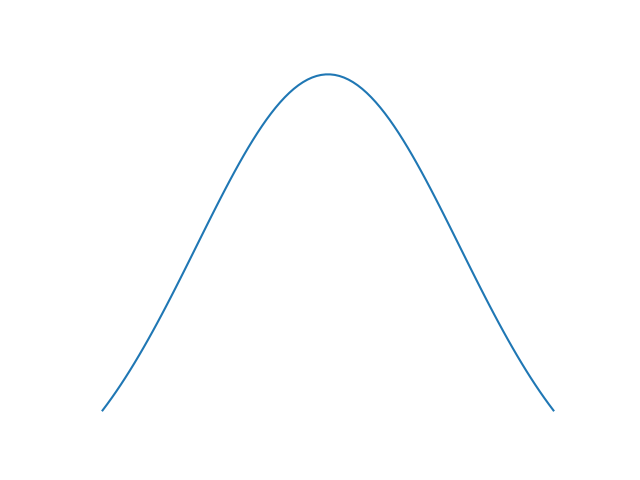
\includegraphics{images/real.png}};
		\node[right=of R,scale=2,draw=black,thick] (F) {\(F\)};
		\only<3>{\node[scale=2,draw=black,thick,fill=VapourCyan!30] at (F) {\(F\)};}
		\node[scale=0.55,right=of F] (S) {
			\begin{tabular}{w|w|w}
				Age & Location & Test scores \\ \hline\hline
				58 & B & \(n_3\) \\
				34 & D & \(n_4\) \\
				78 & A & \(n_1\) \\
				\ldots & \ldots & \ldots
			\end{tabular}
		};
		\node[above=of S,scale=2,yshift=-0.5cm] {\(S\)};
		\node[below=of S,yshift=1cm,scale=0.2] {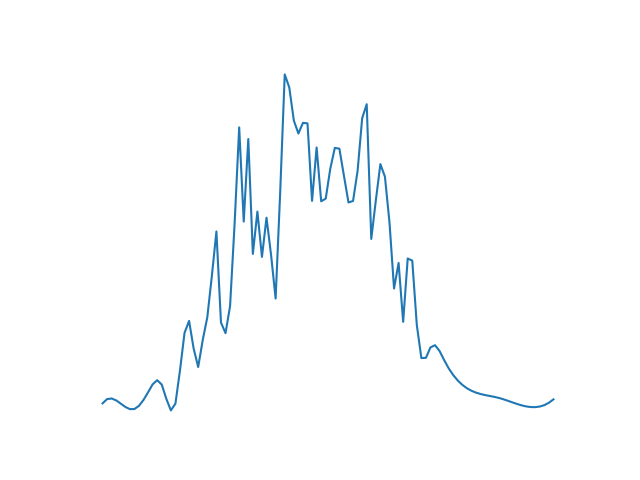
\includegraphics{images/synthetic.png}};
		\only<2->{
			\node[scale=0.55,draw=black,very thick] at (S) {
				\begin{tabular}{w|w|w}
					Age & Location & Test scores \\ \hline\hline
					58 & B & \(n_3\) \\
					34 & D & \(n_4\) \\
					78 & A & \(n_1\) \\
					\ldots & \ldots & \ldots
				\end{tabular}
			};
		}
		\only<4->{
			\node[scale=0.55] at (S) {
				\begin{tabular}{o|o|o}
					Age & Location & Test scores \\ \hline\hline
					58 & B & \(n_3\) \\
					34 & D & \(n_4\) \\
					78 & A & \(n_1\) \\
					\ldots & \ldots & \ldots
				\end{tabular}
			};
		}
		\draw[->,thick,VapourCyan] (R) to [out=0,in=180] node[midway,scale=0.5,above] {Train} (F);
		\draw[->,thick,VapourMagenta] (F) to [out=0,in=180] node[midway,scale=0.5,above] {Sample} (S);
	\end{tikzpicture}
	\bigskip

	\visible<5>{\textbf{\textsc{What is the \hlorangeu{expected privacy gain} from analysing \(S\) instead of \(R\) for different generative models for \(\boxed{F}\)?}}}
	\end{figure}
\end{frame}

\begin{frame}{Key findings}
	\vspace{1cm}
   	\begin{itemize}
   		\setlength\itemsep{2em}
   		\item Synthetic data generators \hlorangeu{do not provide implied privacy guarantees}
   		\begin{itemize}
   			\item little to no benefit over publishing real data
   		\end{itemize}
	   	\item \hlmagenta{Differential privacy} provides little benefits for synthetic data
	   	\item Strong \hlcyan{utility vs privacy} trade-off
   	\end{itemize}
   	\begin{tikzpicture}
   		\node[scale=0.2] (R) {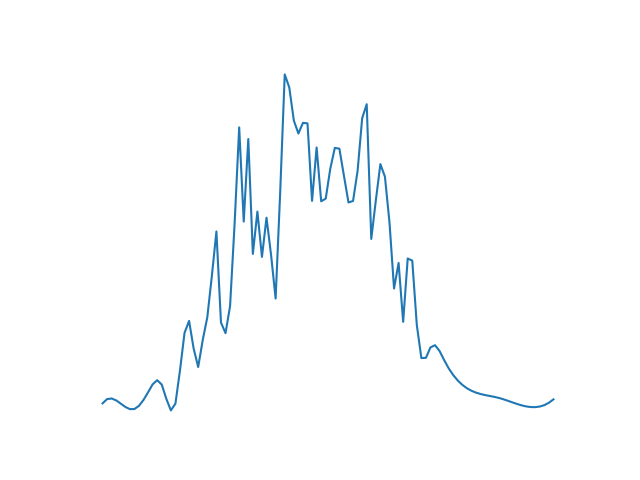
\includegraphics{images/synthetic.png}};
   		\node[right=of S,xshift=-4cm,scale=0.2] (S) {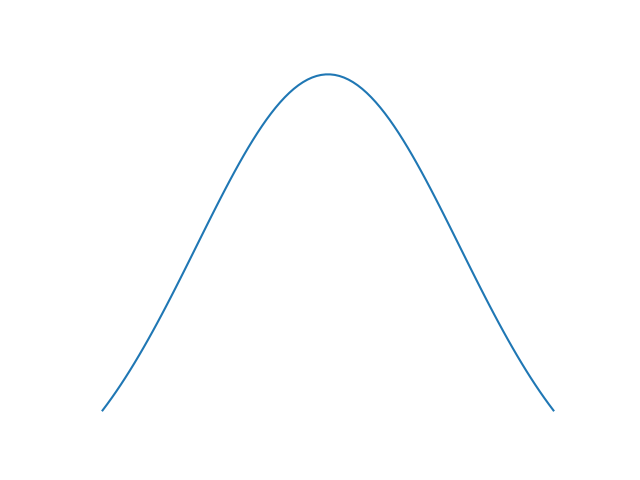
\includegraphics{images/real.png}};
   		\draw[->,thick,black] (R) to [out=0,in=180] node[midway,yshift=0.3cm,scale=0.9,above,draw=VapourCyan,very thick] {privacy \(\rightarrow\) 0} (S);
   	\end{tikzpicture}
\end{frame}

\begin{frame}{Sensitive datasets}
	\vspace{1cm}
    \only<1>{
	    \begin{table}
		    \resizebox{.9\textwidth}{!}{%
				\begin{tabular}{w||w|w|w|w}
				Identity & Age & Location & Test scores & Classification \\ \hline\hline
				Person 1 & 52 & A & \(n_1\) & X \\
				Person 2 & 29 & B & \(n_2\) & Y \\
				Person 3 & 89 & C & \(n_3\) & Z \\
				\ldots & \ldots & \ldots & \ldots & \ldots
				\end{tabular}
			}
		\end{table}
	}
	\only<2-5>{
		\begin{table}
			\resizebox{.9\textwidth}{!}{%
				\begin{tabular}{w||w|w|o|o}
				Identity & Age & Location & Test scores & Classification \\ \hline\hline
				Person 1 & 52 & A & \(n_1\) & X \\
				Person 2 & 29 & B & \(n_2\) & Y \\
				Person 3 & 89 & C & \(n_3\) & Z \\
				\ldots & \ldots & \ldots & \ldots & \ldots
				\end{tabular}
			}
		\end{table}
	}
	\only<6>{
		\begin{table}
			\resizebox{.9\textwidth}{!}{%
				\begin{tabular}{w||w|w|w|w}
				Identity & Age & Location & Test scores & Classification \\ \hline\hline
				\rowcolor{VapourCyan!30}Person 1 & 52 & A & \(n_1\) & X \\
				Person 2 & 29 & B & \(n_2\) & Y \\
				Person 3 & 89 & C & \(n_3\) & Z \\
				\ldots & \ldots & \ldots & \ldots & \ldots
				\end{tabular}
			}
		\end{table}
	}\bigskip
	\visible<3->{\centertitle{Hiding sensitive data}}
	\begin{itemize}
		\item<3-> Companies
		\item<4-> Employers
		\item<5-> Governments
	\end{itemize}
\end{frame}

\begin{frame}{Privacy tradeoffs}
	\vspace{1cm}
    \only<1>{
		\begin{table}
			\resizebox{.9\textwidth}{!}{%
				\begin{tabular}{w||w|w|o|o}
				Identity & Age & Location & Test scores & Classification \\ \hline\hline
				Person 1 & 52 & A & \(n_1\) & X \\
				Person 2 & 29 & B & \(n_2\) & Y \\
				Person 3 & 89 & C & \(n_3\) & Z \\
				\ldots & \ldots & \ldots & \ldots & \ldots
				\end{tabular}
			}
		\end{table}
	}
	\only<2>{
		\begin{table}
		    \resizebox{.9\textwidth}{!}{%
				\begin{tabular}{w||w|w|x|x}
				Identity & Age & Location & Test scores & Classification \\ \hline\hline
				Person 1 & 52 & A & \textbf{?} & \textbf{?} \\
				Person 2 & 29 & B & \textbf{?} & \textbf{?} \\
				Person 3 & 89 & C & \textbf{?} & \textbf{?} \\
				\ldots & \ldots & \ldots & \ldots & \ldots
				\end{tabular}
			}
		\end{table}
	}
	\only<3->{
		\begin{table}
		    \resizebox{.9\textwidth}{!}{%
				\begin{tabular}{y||v|v|w|w}
				Identity & Age & Location & Test scores & Classification \\ \hline\hline
				ID 1 & 52 & A & \(n_1\) & X \\
				ID 2 & 29 & B & \(n_2\) & Y \\
				ID 3 & 89 & C & \(n_3\) & Z \\
				\ldots & \ldots & \ldots & \ldots & \ldots
				\end{tabular}
			}
		\end{table}
	}
	\bigskip

	\begin{itemize}
		\item<1-> Releasing such \hlorangeu{data} harms privacy of individuals
		\item<2-> Removing \hlcyan{columns} harms utility
		\item<3-> Removing \hlblue{names} can help, but \hlmagenta{identifying data} still exists
	\end{itemize}
\end{frame}

\begin{frame}{Security requirements :: page \small{2}}
	\vspace{1cm}
	\only<1-2>{
		\begin{table}
			\resizebox{.9\textwidth}{!}{%
				\begin{tabular}{w||w|w|w|w}
				Identity & Age & Location & Test scores & Classification \\ \hline\hline
				Person 1 & 52 & A & \(n_1\) & X \\
				Person 2 & 29 & B & \(n_2\) & Y \\
				Person 3 & 89 & C & \(n_3\) & Z \\
				\ldots & \ldots & \ldots & \ldots & \ldots
				\end{tabular}
			}
		\end{table}
	}
	\only<3>{
		\begin{table}
			\resizebox{.9\textwidth}{!}{%
				\begin{tabular}{w||w|w|w|w}
				Identity & Age & Location & Test scores & Classification \\ \hline\hline
				\rowcolor{VapourCyan!30}Person 1 & 52 & A & \(n_1\) & X \\
				Person 2 & 29 & B & \(n_2\) & Y \\
				Person 3 & 89 & C & \(n_3\) & Z \\
				\ldots & \ldots & \ldots & \ldots & \ldots
				\end{tabular}
			}
		\end{table}
	}
	\only<4>{
		\begin{table}
			\resizebox{.9\textwidth}{!}{%
				\begin{tabular}{w||w|w|w|w}
				Identity & Age & Location & Test scores & Classification \\ \hline\hline
				\rowcolor{VapourCyan!30}? & 52 & A & \(n_1\) & X \\
				? & 29 & B & \(n_2\) & Y \\
				? & 89 & C & \(n_3\) & Z \\
				\ldots & \ldots & \ldots & \ldots & \ldots
				\end{tabular}
			}
		\end{table}
	}
	\only<5>{
		\begin{table}
			\resizebox{.9\textwidth}{!}{%
				\begin{tabular}{w||w|w|v|v}
				\rowcolor{white}Identity & Age & Location & Test scores & Classification \\ \hline\hline
				? & 52 & A & \hlmagenta{\(n_1\)} & \hlmagenta{X} \\
				\rowcolor{white}? & 29 & B & \(n_2\) & Y \\
				\rowcolor{white}? & 89 & C & \(n_3\) & Z \\
				\rowcolor{white}\ldots & \ldots & \ldots & \ldots & \ldots
				\end{tabular}
			}
		\end{table}
	}
	\bigskip

	\begin{itemize}
		\setlength\itemsep{2em}
		\item<1-> The adversary is modelled as an algorithm \(\adv\) that attempts to learn from synthetic data generator outputs
		\item<2-> \cite{Arxiv:SOT21} models the following \textit{attacks} based on GDPR \textit{\textbf{linkage}} properties
		\begin{itemize}
			\item<3-> \hlcyan{Membership inference}: was an individual a \textbf{member} of the original dataset?
			\item<5-> \hlmagenta{Attribute inference}: can a sensitive individual \textbf{attribute} be inferred?
		\end{itemize}
	\end{itemize}
\end{frame}

\begin{frame}{Privacy: k-anonymity}
	\vspace{1cm}
	\only<1-2>{
		\begin{table}
		    \resizebox{.9\textwidth}{!}{%
				\begin{tabular}{w|w|w|w}
				Age & Location & Test scores & Classification \\ \hline\hline
				25-40 & A & \(x < n_1\) & X \\
				25-40 & B & \(x < n_1\) & Y \\
				25-40 & B & \(n_1 < x < n_2\) & Z \\
				40-55 & B & \(n_1 < x < n_2\) & W \\
				40-55 & C & \(n_1 < x < n_2\) & U \\
				\ldots & \ldots & \ldots & \ldots
				\end{tabular}
			}
		\end{table}
	}
	\only<3>{
		\begin{table}
		    \resizebox{.9\textwidth}{!}{%
				\begin{tabular}{w|w|w|w}
				Age & Location & Test scores & Classification \\ \hline\hline
				25-40 & A & \(x < n_1\) & X \\
				25-40 & B & \(x < n_1\) & Y \\
				25-40 & B & \(n_1 < x < n_2\) & Z \\
				\rowcolor{VapourMagenta!20}
				40-55 & B & \(n_1 < x < n_2\) & W \\
				\rowcolor{VapourMagenta!20}
				40-55 & C & \(n_1 < x < n_2\) & U \\
				\ldots & \ldots & \ldots & \ldots
				\end{tabular}
			}
		\end{table}
	}
	\bigskip

	\begin{itemize}
		\item<1-> Each line corresponds to \(k\) identities
		\item<2-> \textbf{Problem}: does not provide concrete privacy guarantees
		\item<3-> \textbf{Example}: Anyone in \hlmagenta{40-55} must have a test score between \(n_1\) and \(n_2\), etc.
	\end{itemize}
\end{frame}

\begin{frame}{Objective}
	\vspace{1cm}
	\begin{figure}
	\begin{tikzpicture}
		\node[scale=0.6] (R) {
			\begin{tabular}{w|w|w}
			Age & Location & Test scores \\ \hline\hline
			52 & A & \(n_1\) \\
			\rowcolor{VapourCyan!30}29 & B & \(n_2\) \\
			89 & C & \(n_3\) \\
			\ldots & \ldots & \ldots
			\end{tabular}
		};
		\node[above=of R,scale=2,yshift=-0.5cm] {\(D_1\)};
		\node[scale=0.6,right=of R] (S) {
			\begin{tabular}{w|w|w}
				Age & Location & Test scores \\ \hline\hline
				52 & A & \(n_1\) \\
				\rowcolor{VapourCyan!30}34 & D & \(n_2\) \\
				89 & C & \(n_3\) \\
				\ldots & \ldots & \ldots
			\end{tabular}
		};
		\node[above=of S,scale=2,yshift=-0.5cm] {\(D_2\)};
	\end{tikzpicture}
	\bigskip

	\(\forall D_2\) that differs with \(D_1\) on \hlcyan{one row}, and some query \(Q\):
	\begin{equation}
	\prob{d \leftarrow Q(D_1)} \leq e^\epsilon\prob{d \leftarrow Q(D_2)}
	\label{eq:dp}
	\end{equation}
	\begin{itemize}
		\item<2-> For small \(\epsilon\), \(e^\epsilon \approx 1+\epsilon\)
		\item<3> As \(\epsilon \rightarrow 0\), probabilities in \eqref{eq:dp} become closer 
	\end{itemize}
	\end{figure}
\end{frame}

\begin{frame}{Privacy: differential privacy}
	\vspace{1cm}
	\only<1>{
		\textsc{Real dataset} \(R\)
		\begin{table}
		    \resizebox{.9\textwidth}{!}{%
				\begin{tabular}{w||w|w|w|w}
				Identity & Age & Location & Test scores & Classification \\ \hline\hline
				ID 1 & 52 & A & \(n_1\) & X \\
				ID 2 & 29 & B & \(n_2\) & Y \\
				ID 3 & 89 & C & \(n_3\) & Z \\
				\ldots & \ldots & \ldots & \ldots & \ldots
				\end{tabular}
			}
		\end{table}
	}
	\only<2->{
		\textsc{Real dataset} \(R\)
		\begin{table}
		    \resizebox{.9\textwidth}{!}{%
				\begin{tabular}{w||y|w|x|w}
				Identity & Age & Location & Test scores & Classification \\ \hline\hline
				ID 1 & 52 & A & \(n_1\) & X \\
				ID 2 & 29 & B & \(n_2\) & Y \\
				ID 3 & 89 & C & \(n_3\) & Z \\
				\ldots & \ldots & \ldots & \ldots & \ldots
				\end{tabular}
			}
		\end{table}
	}
	\visible<2->{\footnotesize{\(Q_{\text{\#},R}\) = \(\textsc{Count}_R\)(\hlblue{(\textsc{Age} \(>\) 50)} \(\wedge\) \hlcyan{(\textsc{Test score} $> n_4$)}))}}\\\bigskip
	\visible<3->{\footnotesize{\textsc{Publish} [\(Q_{\text{\#},R}\) + \tikzmark{noisestart}Noise(\tikzmark{epszstart}\(\epsilon_{f}\)\tikzmark{epszend}, \tikzmark{sensstart}\(\Delta Q_{\#,R}\)\tikzmark{sensend})\tikzmark{noiseend}}]}
	\bigskip

	\begin{itemize}
		\item<1-> \textbf{Idea}: limit access to table and add noise to query outputs
		\item<7-> \tikzmark{totallossstart}\textbf{Problem}\tikzmark{totallossend}: privacy loss accumulates for each query \(q\)
	\end{itemize}

	\visible<4>{
		\begin{tikzpicture}[overlay, remember picture]
		  \draw [->,thick,VapourCyan] (epszstart.south) -- (epszend.south) to[out=270,in=180] ++ (1.5,-0.2) node[right,scale=0.7] {\textbf{privacy parameter} (\(\text{[}\epsilon_z \rightarrow 0\text{]} \Rightarrow\) [privacy \(\rightarrow \infty\)])};
		\end{tikzpicture}
	}
	\visible<5>{
		\begin{tikzpicture}[overlay, remember picture]
		  \draw [->,thick,VapourCyan] (sensstart.south) -- (sensend.south) to[out=270,in=180] ++ (1,0) node[right,scale=0.8]{\textbf{sensitivity} (\(\max_{R_1,R_2} \|Q_{\#,R_1} - Q_{\#,R_2}\|\))};
		\end{tikzpicture}
	}
	\visible<6>{
		\begin{tikzpicture}[overlay, remember picture]
		  \draw [->,thick,VapourCyan] (noisestart.south) -- (noiseend.south) to[out=270,in=180] ++ (0.5,0) node[right,text width=6cm] (laplace) {e.g. sample from Lap(\(\Delta Q_z/\epsilon\)) \(= \frac{\epsilon}{2\Delta Q_z} * \exp(-\epsilon|x|/\Delta Q_z)\)};
		\end{tikzpicture}
	}
	\visible<7>{
		\begin{tikzpicture}[overlay, remember picture]
		  \draw [->,thick,VapourCyan] (totallossstart.south) -- (totallossend.south) to[out=270,in=180] ++ (1,-0.5) node[right]{the \textbf{total loss} is roughly \(\epsilon = \sum_{q \in \mathcal{Q}} \epsilon_q\)};
		\end{tikzpicture}
	}
\end{frame}

\section{Synthetic data}
\begin{frame}{Generative models :: section IV.A}
	\vspace{1cm}
	\begin{figure}
	\begin{tikzpicture}
		\node[scale=0.55] (R) {
			\begin{tabular}{w|w|w}
			Age & Location & Test scores \\ \hline\hline
			52 & A & \(n_1\) \\
			29 & B & \(n_2\) \\
			89 & C & \(n_3\) \\
			\ldots & \ldots & \ldots
			\end{tabular}
		};
		\node[above=of R,scale=2,yshift=-0.5cm] {\(R\)};
		\node[right=of R,scale=2,draw=black,thick] (F) {\(\texttt{GM}\)};
		\node[scale=0.55,right=of F] (S) {
			\begin{tabular}{w|w|w}
				Age & Location & Test scores \\ \hline\hline
				58 & B & \(n_1\) \\
				34 & D & \(n_2\) \\
				78 & A & \(n_3\) \\
				\ldots & \ldots & \ldots
			\end{tabular}
		};
		\node[above=of S,scale=2,yshift=-0.5cm] {\(S\)};
		\draw[->,thick,VapourCyan] (R) to [out=0,in=180] node[midway,scale=0.5,above] {Train} (F);
		\draw[->,thick,VapourMagenta] (F) to [out=0,in=180] node[midway,scale=0.5,above] {Sample} (S);
		\node[below=of F,text width=8cm,draw=orangeu,very thick] (T) {\textcolor{orangeu}{The generative model \textcolor{VapourCyan}{\texttt{GM}} `learns' the distribution of \(R\) and then samples new records to create \(S\)}};
		\draw[->,thick,orangeu] (F) -- (T);
	\end{tikzpicture}
	\end{figure}
\end{frame}

\begin{frame}{Generative models :: section IV.A}
   \vspace{1cm}
	\begin{figure}
	\centering
	\scalebox{1.5}{
		\begin{tikzpicture}
		\node (X) {\(R\)};
		\node[right=of X,thick,draw=VapourCyan] (GM) {\(\texttt{GM}\)};
		\node[right=of GM] (GMX) {\(\texttt{GM}(X)\)};
		\node[right=of GMX,xshift=-1cm] (sim) {\(\sim\)};
		\node[right=of sim,xshift=-1cm] (S) {\(S\)};
		\draw[->, thick] (X) -- (GM) -- (GMX);
		\end{tikzpicture}
	}
	\end{figure}\bigskip
	\visible<2->{
   		This work considers three fundamental approaches: 
   		\begin{itemize}
   			\item Independent histograms (\textbf{IndHist})
   			\item Bayes networks (\textbf{BayNet})
   			\item Generative adversarial networks (\textbf{GANs})
   		\end{itemize}
    }
\end{frame}

\begin{frame}{IndHist :: page \small{4}}
   \vspace{1cm}
	\begin{figure}
	\centering
	\scalebox{1.5}{
		\begin{tikzpicture}
		\node (X) {\(R\)};
		\node[right=of X,thick,draw=VapourCyan] (GM) {\(\texttt{GM}\)};
		\node[right=of GM] (GMX) {\(\texttt{GM}(X)\)};
		\draw[->, thick] (X) -- (GM) -- (GMX);
		\node[right=of GMX,scale=0.3,xshift=-1cm] (R1) {
			\begin{tabular}{|x|y|v|o|} \hline
			Age & Locale & Score & Class \\ \hline\hline
			& & & \\ \hline
			& & & \\ \hline
			& & & \\ \hline
			& & & \\ \hline
			\end{tabular}
		};
		\end{tikzpicture}
	}
	\end{figure}\bigskip
	{\Large{\(\boxed{\texttt{GM}(X)}\)}}:
	\small{\begin{itemize}
			\item A set of independent histograms for each column in dataset
			\item Sample synthetic records by sampling a value from the probability distribution of each histogram independently
		\end{itemize}}
\end{frame}

\begin{frame}{BayNet :: page \small{4}}
   \vspace{1cm}
	\begin{figure}
	\centering
	\scalebox{1.5}{
		\begin{tikzpicture}
		\node (X) {\(R\)};
		\node[right=of X,thick,draw=VapourCyan] (GM) {\(\texttt{GM}\)};
		\node[right=of GM] (GMX) {\(\texttt{GM}(X)\)};
		\draw[->, thick] (X) -- (GM) -- (GMX);
		\node[right=of GMX,xshift=-0.8cm,scale=0.4] (BayNet) {
			\begin{tikzpicture}
			\node[draw=black,circle,fill=VapourCyan!30] (Age) {\(Age\)};
			\node[draw=black,circle,fill=VapourMagenta!20,right=of Age] (Score) {\(Score\)};
			\node[draw=black,circle,fill=orangeu!30,below right=of Age] (Class) {\(Class\)};
			\node[draw=black,circle,fill=LightBlue!60,below left=of Age] (Locale) {\(Locale\)};
			\draw[->,very thick] (Age) -- (Score);
			\draw[->,very thick] (Age) -- (Locale);
			\draw[->,very thick] (Locale) -- (Class);
			\draw[->,very thick] (Locale) -- (Score);
			\draw[->,very thick] (Score) -- (Class);
			\end{tikzpicture}
		};
		\end{tikzpicture}
	}
	\end{figure}\bigskip
	\Large{\(\boxed{\texttt{GM}(X)}\)}:
	\small{\begin{itemize}
			\item A graph that models conditional probabilities relationships of attributes
			\item Samples synthetic records by sampling from \hlcyan{root nodes} and traversing network and sampling from conditional probabilities
		\end{itemize}}
\end{frame}

\begin{frame}{CTGAN :: page \small{5}}
   \vspace{1cm}
	\begin{figure}
	\centering
	\scalebox{1.5}{
		\begin{tikzpicture}
		\node (X) {\(R\)};
		\node[right=of X,thick,draw=VapourCyan] (GM) {\(\texttt{GM}\)};
		\node[right=of GM] (GMX) {\(\texttt{GM}(X)\)};
		\draw[->, thick] (X) -- (GM) -- (GMX);
		\end{tikzpicture}
	}
	\end{figure}\bigskip
	\Large{\(\boxed{\texttt{GM}(X)}\)}:
	\small{\begin{itemize}
			\setlength\itemsep{2em}
			\item Uses \textbf{CTGAN}~\cite{CTGAN} (non-parametric) approach to learn data distribution of dataset
			\item Process probabilistically trains a simulator that produces synthetic records that a \textit{discriminator} algorithm cannot distinguish from real records.
			\item Preserved characteristics distribution of are not known \textbf{until} training
		\end{itemize}}
\end{frame}

\begin{frame}{Differentially private generators}
   \vspace{1cm}
   \begin{itemize}
   	\setlength\itemsep{3em}
   	\item Consider an additional two generators: \textbf{PrivBayes}, \textbf{PATEGAN}~\cite{PATEGAN}
   	\item Both learn data distributions under algorithms that inject noise into conditional probability queries during \textbf{BayNet} and \textbf{CTGAN} training
   	\item Sampling records from \(\texttt{GM}(X)\) does not use additional privacy budget
   \end{itemize}
\end{frame}

\section{Privacy gain}

\begin{frame}{Privacy loss :: III.A, page {\small 3}}
	\vspace{1cm}
	\begin{figure}
	\centering
	\scalebox{1.5}{
		\begin{tikzpicture}
		\node (X) {\(X\)};
		\node[right=of X,xshift=-1cm] (sim) {\(\sim\)};
		\node[right=of sim,xshift=-1cm] (A) {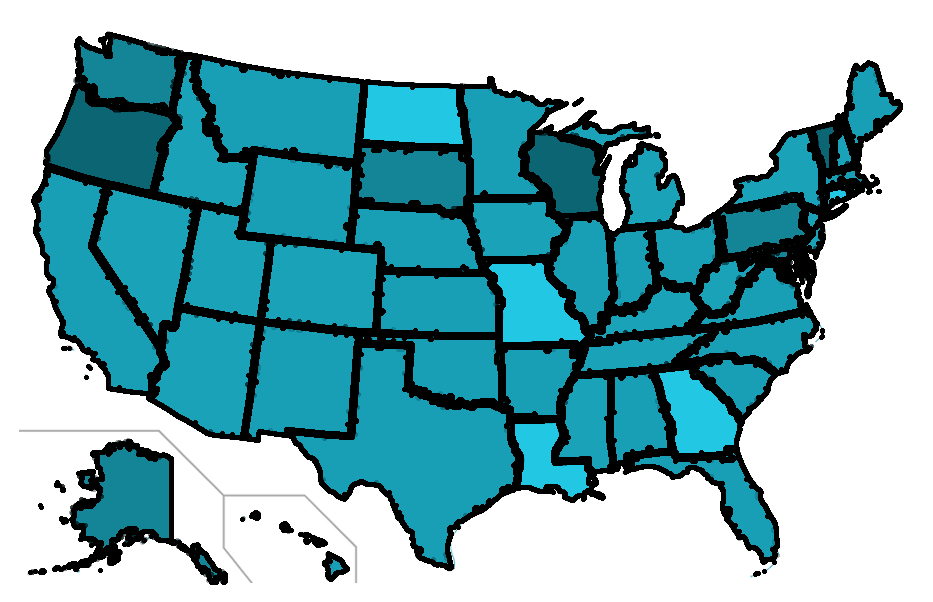
\includegraphics[scale=0.05]{images/heatmap-alt.png}};
		\node[right=of A] (B) {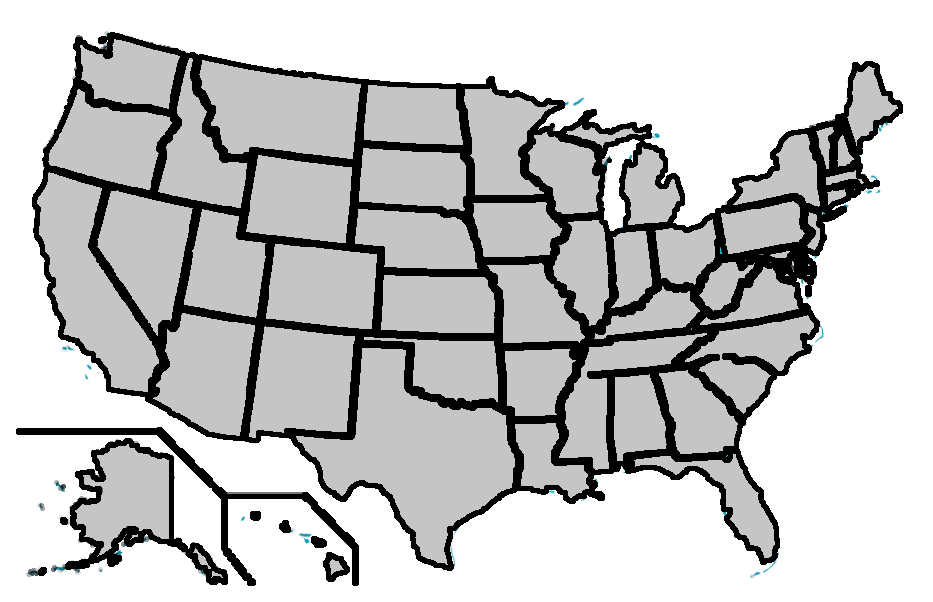
\includegraphics[scale=0.05]{images/heatmap-gray.png}};
		\node[right=of B,xshift=-1cm] (R) {\R};
		\draw[->, thick] (B) -- node[midway, above] {\(\D\)} (A);
		\end{tikzpicture}
	}
	\end{figure}
	
	\visible<2->{
	    \begin{itemize}
	    	\item<2-> Select a person \(\bm{t} \in \R\)
	    	\item<3-> Let \(t_s \sim \bm{t}\) be a \textbf{secret} associated with \(\bm{t}\)
	    	\item<3-> The \textbf{privacy loss} for \(X\) is defined as:
	    	\[
	    	\privloss{X} = \prob{\widehat{t_s} = t_s | X} - \prob{t_s} \only<4>{= \hlorangeu{1 - 0}}\only<5>{= \hlcyan{0 - 1}}
	    	\]
	    	where \(\widehat{t_s}\) is the guess of the adversary.
	    	\item<4-> \hlorangeu{\(\privloss{X} = 1\)} implies \textbf{total loss} of privacy.
	    	\item<5-> \hlcyan{\(\privloss{X} = -1\)} implies \textbf{perfect privacy}.
	    \end{itemize}
    }
\end{frame}

\begin{frame}{Privacy gain :: III.A, page {\small 4}}
	\vspace{1cm}
    \begin{itemize}
    	\setlength\itemsep{2em}
    	\item The \textbf{privacy gain} from using \(X_2\) instead of \(X_1\) is:
    	\[
    	\privgain{X_2,X_1} = \frac{\privloss{X_1} - \privloss{X_2}}{2}.
    	\]
    	\item<2-> \(\privgain{X_2,X_1} > 0\) implies \(X_2\) preserves more privacy, and vice-versa.
    \end{itemize}
\end{frame}

\section{Privacy analysis}

\begin{frame}{Experimental setup :: section IV.B}
	\vspace{1cm}
    \begin{itemize}
    	\setlength\itemsep{2em}
    	\item Three datasets: Texas, Adult, German
    	\item Evaluate expected privacy gains for each of the five generative models under \tikzmark{wcstart}\textbf{worst-case}\tikzmark{wcend} and \tikzmark{acstart}\textbf{average-case}\tikzmark{acend} analyses
    \end{itemize}
    \begin{tikzpicture}[overlay,remember picture]
		\draw<2>[->,thick,VapourCyan] (wcstart.south) -- (wcend.south) to[out=0,in=0] ++ (-2,-2) node[left,text width=8cm,scale=0.7] {Craft a target individual with each attribute set to least likely column value};
		\draw<3>[->,thick,VapourCyan] (acend.south) -- (acstart.south) to[out=180,in=180] ++ (0,-1.5) node[right,text width=10cm,scale=0.7,draw=VapourCyan,very thick] {
			For each dataset, repeat \(n_R\) times:
			\begin{itemize}
				\item Sample a random set of \(T\) targets from the datasets
				\item Sample \(n_S\) synthetic datasets
				\item Evaluate average privacy gain across all \(n_S\) datasets
			\end{itemize}\bigskip
		};
	\end{tikzpicture}
\end{frame}

\begin{frame}{Attribute inference :: section V}
	\centertitle{Train (algorithm 1)}
	Repeat \(n_S\) times:
	\begin{figure}
	\begin{tikzpicture}
		\node[scale=0.55] (R) {
			\begin{tabular}{|w|w|w|w|w|w|w||o|} \hline
			\multicolumn{7}{|c||}{\(\texttt{R}_k\)} & \(\bm{r}_s\) \\ \hline\hline
			& & & & & & & \\ \hline
			& & & & & & & \\ \hline
			& & & & & & & \\ \hline
			& & & & & & & \\ \hline
			& & & & & & & \\ \hline
			& & & & & & & \\ \hline
			\end{tabular}
		};
		\node[above=of R,yshift=-1cm] {\(\texttt{R}_t\)};
		\node[right=of R,xshift=2cm,scale=0.55] (S) {
			\begin{tabular}{|w|w|w|w|w|w|w||o|} \hline
			\multicolumn{7}{|c||}{\(\texttt{R}_k\)} & \(\bm{r}_s\) \\ \hline\hline
			& & & & & & & \\ \hline
			& & & & & & & \\ \hline
			& & & & & & & \\ \hline
			& & & & & & & \\ \hline
			& & & & & & & \\ \hline
			& & & & & & & \\ \hline
			\end{tabular}
		};
		\node[above=of S,yshift=-1cm] {\(\texttt{S}_t\)};
		\draw[->,thick] (R) to[out=0,in=180] node[midway,above] {\(\texttt{GM}(\texttt{R})\)} (S);
		\visible<2->{
			\node[below=of R,yshift=0.5cm,draw=black,very thick] (LRR) {\(LinReg(\texttt{R})\)};
			\node[below=of S,yshift=0.5cm,draw=black,very thick] (LRS) {\(LinReg(\texttt{S})\)};
			\draw[->,thick] (R) -- (LRR);
			\draw[->,thick] (S) -- (LRS);
		}
	\end{tikzpicture}
	\end{figure}
\end{frame}

\begin{frame}{Attribute inference :: section V}
	\centertitle{Infer (algorithm 2)}
	\begin{figure}
	\begin{tikzpicture}
		\only<1>{
			\node[scale=0.55] (R) {
				\begin{tabular}{|w|w|w|w|w|w|w||o|} \hline
				\multicolumn{7}{|c||}{\(\texttt{R}_k\)} & \(\bm{r}_s\) \\ \hline\hline
				\rowcolor{white} & & & & & & & \\ \hline
				\rowcolor{white} & & & & & & & \\ \hline
				\rowcolor{VapourCyan!30}\multicolumn{7}{|c||}{\(\bm{t}_k\)} & \hlorangeu{\(t_s\)} \\ \hline
				\rowcolor{white} & & & & & & & \\ \hline
				\rowcolor{white} & & & & & & & \\ \hline
				\rowcolor{white} & & & & & & & \\ \hline
				\end{tabular}
			};
			\node[above=of R,yshift=-1cm] {\(\texttt{R}\)};
		}
		\only<2->{
			\node[scale=0.55] (R) {
				\begin{tabular}{|w|w|w|w|w|w|w|} \hline
				\multicolumn{7}{|c|}{\(\texttt{R}_k\)} \\ \hline\hline
				& & & & & & \\ \hline
				& & & & & & \\ \hline
				\rowcolor{VapourCyan!30}\multicolumn{7}{|c|}{\(\bm{t}_k\)} \\ \hline
				& & & & & & \\ \hline
				& & & & & & \\ \hline
				& & & & & & \\ \hline
				\end{tabular}
			};
			\node[above=of R,yshift=-1cm] {\(\texttt{R}\)};
		}
		\visible<2->{
			\node[below left=of R,yshift=0.5cm,draw=black,very thick] (LRR) {\(LinReg(\texttt{R})\lbrack\bm{t_k}\rbrack\)};
			\node[below right=of R,yshift=0.5cm,draw=black,very thick] (LRS) {\(LinReg(\texttt{S})\lbrack\bm{t_k}\rbrack\)};
			\node[below=of LRR,yshift=0.5cm] (tR) {\(\widehat{t_s}\)};
			\node[below=of LRS,yshift=0.5cm] (tS) {\(\widehat{t_s}\)};
			\draw[->,thick] (R) -- (LRR) -- (tR);
			\draw[->,thick] (R) -- (LRS) -- (tS);
		}
	\end{tikzpicture}
	\end{figure}
	\bigskip

	\visible<3>{\textbf{Privacy gain}: \(\prob{\widehat{t}_s = t_s | \texttt{S}} - \prob{\widehat{t}_s = t_s | \texttt{R}}\)}
\end{frame}

\begin{frame}{Membership inference :: section VI}
	\centertitle{Train (algorithm 3)}
	Repeat \(n_S\) times:
	\begin{figure}
	\begin{tikzpicture}
		\node[scale=0.55] (R1) {
			\begin{tabular}{|w|w|w|w|w|w|w|w|} \hline
			& & & & & & & \\ \hline
			& & & & & & & \\ \hline
			& & & & & & & \\ \hline
			& & & & & & & \\ \hline
			& & & & & & & \\ \hline
			& & & & & & & \\ \hline
			& & & & & & & \\ \hline
			\end{tabular}
		};
		\node[scale=0.55,below=of R1] (R2) {
			\begin{tabular}{|w|w|w|w|w|w|w|w|} \hline
			& & & & & & & \\ \hline
			& & & & & & & \\ \hline
			& & & & & & & \\ \hline
			\rowcolor{VapourCyan!30}\multicolumn{8}{|c|}{\(\bm{t}\)} \\ \hline
			& & & & & & & \\ \hline
			& & & & & & & \\ \hline
			& & & & & & & \\ \hline
			\end{tabular}
		};
		\visible<2->{\node[right=of R1,scale=0.55] (S1) {
			\begin{tabular}{|w|w|w|w|w|w|w|w|} \hline
			& & & & & & & \\ \hline
			& & & & & & & \\ \hline
			& & & & & & & \\ \hline
			& & & & & & & \\ \hline
			& & & & & & & \\ \hline
			& & & & & & & \\ \hline
			& & & & & & & \\ \hline
			\end{tabular}
		};}
		\visible<2->{\node[scale=2] at (S1) {\(\texttt{S}_1\)};}
		\visible<2->{\node[right=of R2,scale=0.55] (S2) {
			\begin{tabular}{|w|w|w|w|w|w|w|w|} \hline
			& & & & & & & \\ \hline
			& & & & & & & \\ \hline
			& & & & & & & \\ \hline
			& & & & & & & \\ \hline
			& & & & & & & \\ \hline
			& & & & & & & \\ \hline
			& & & & & & & \\ \hline
			\end{tabular}
		};}
		\visible<2->{\node[scale=2] at (S2) {\(\texttt{S}_2\)};}
		\visible<3>{\node[xshift=3cm,draw=black,very thick] at ($(S1)!0.5!(S2)$) (MIA) {\(\mathcal{MIA}(\texttt{S}_i)\)};}
		\visible<2->{\draw[->,thick] (R1) -- node[midway,above] {\texttt{GM}} (S1);}
		\visible<2->{\draw[->,thick] (R2) -- node[midway,above] {\texttt{GM}} (S2);}
		\visible<3>{\draw[->,thick] (S1) -- (MIA);}
		\visible<3>{\draw[->,thick] (S2) -- (MIA);}
	\end{tikzpicture}
	\end{figure}
\end{frame}

\begin{frame}{Membership inference :: section VI}
	\centertitle{Infer (algorithm 4)}
	\begin{figure}
	\begin{tikzpicture}
		\node[scale=0.55] (R1) {
			\begin{tabular}{|w|w|w|w|w|w|w|w|} \hline
			& & & & & & & \\ \hline
			& & & & & & & \\ \hline
			& & & & & & & \\ \hline
			& & & & & & & \\ \hline
			& & & & & & & \\ \hline
			& & & & & & & \\ \hline
			& & & & & & & \\ \hline
			\end{tabular}
		};
		\node[scale=2] at (R1) {\texttt{?}};
		\node[right=of R1,scale=0.55] (S1) {
			\begin{tabular}{|w|w|w|w|w|w|w|w|} \hline
			& & & & & & & \\ \hline
			& & & & & & & \\ \hline
			& & & & & & & \\ \hline
			& & & & & & & \\ \hline
			& & & & & & & \\ \hline
			& & & & & & & \\ \hline
			& & & & & & & \\ \hline
			\end{tabular}
		};
		\node[scale=2] at (S1) {\(\texttt{S}_1\)};
		\node[right=of S1,draw=black,very thick] (MIA) {\(\mathcal{MIA}(\texttt{S}_i)\)};
		\draw[->,thick] (R1) -- node[midway,above] {\texttt{GM}} (S1);
		\draw[->,thick] (S1) -- (MIA);
		\visible<2->{
			\node[below=of MIA,draw=black,very thick,scale=2] (b) {1/0};
			\draw[->,thick] (MIA) -- (b);
		}
	\end{tikzpicture}
	\end{figure}
\end{frame}

\begin{frame}{Membership inference :: section VI}
    \centertitle{Privacy gain}
    \begin{itemize}
    	\item Privacy gain is:
    	\[
    		\privgain{S,X} = \frac{\privloss{X} - \privloss{S}}{2} \only<2->{ = \hlcyan{(1 - \privloss{S})/2}}
    	\]
    	\item<2-> \textbf{Page 9}: Publishing \(X\) leads to immediate privacy loss, \hlcyan{implies \(\privloss{X} = 1\)}
    	\item<3-> \(\privgain{S,X} = 0.5\) implies \(S\) preserves privacy (\hlcyan{when \(\privloss{S} = 0\)})
    	\item<4-> \(\privgain{S,X} = 0.25\) implies \(S\) neither protects nor reveals secrets (\hlcyan{\(\privloss{S} = 0.5\)} from prior)
    \end{itemize}
\end{frame}

\section{Results}
\begin{frame}{Attribute Inference :: V.D, page {\small 7}}
	\begin{figure}
	\centering
	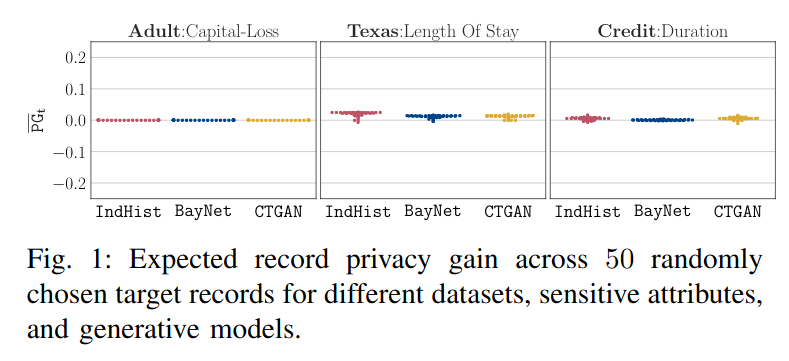
\includegraphics[scale=0.35]{images/fig1.png}
	\end{figure}
\end{frame}

\begin{frame}{Attribute Inference :: V.D, page {\small 7}}
	\begin{figure}
	\centering
	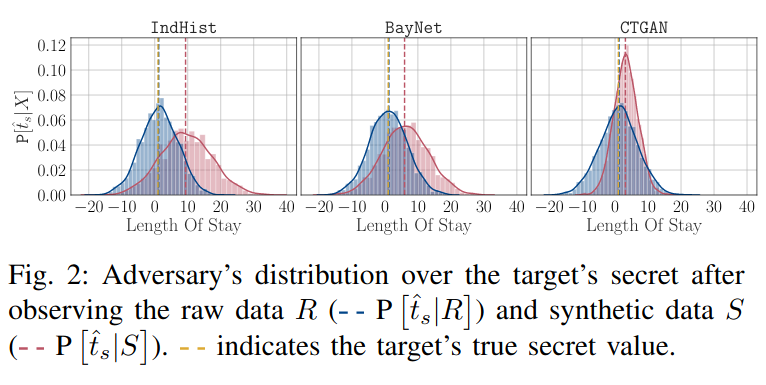
\includegraphics[scale=0.35]{images/fig2.png}
	\end{figure}
\end{frame}

\begin{frame}{Attribute Inference :: V.D, page {\small 8}}
	\vspace{1cm}
	\begin{figure}
	\centering
	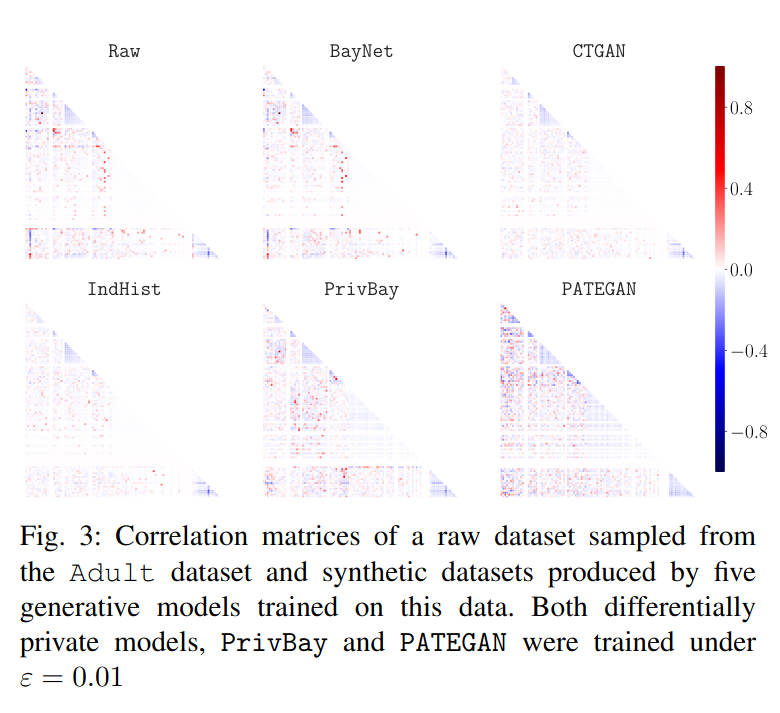
\includegraphics[scale=0.3]{images/fig3.png}
	\end{figure}
\end{frame}

\begin{frame}{Membership Inference :: VI.D, page {\small 10}}
    \begin{figure}
	\centering
	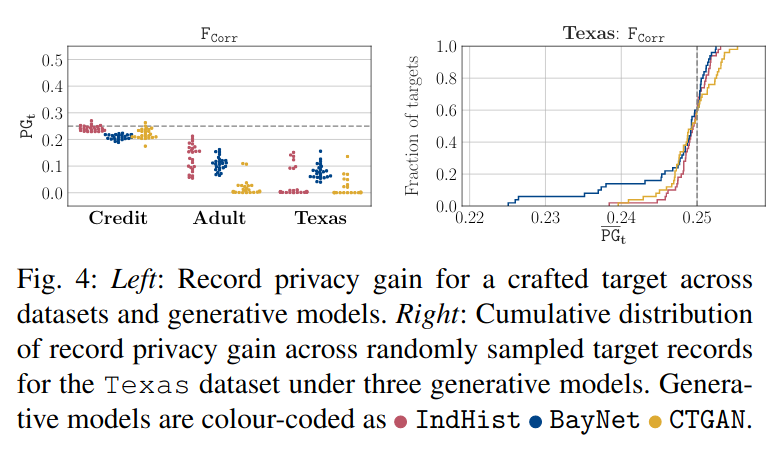
\includegraphics[scale=0.35]{images/fig4.png}
	\end{figure}
\end{frame}

\begin{frame}{Differential privacy :: VII.A}
	\vspace{1cm}
	\centertitle{Attribute inference}
	\begin{figure}
	\centering
	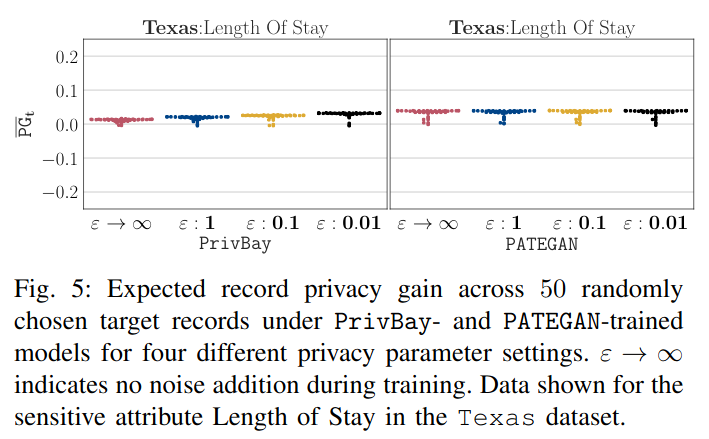
\includegraphics[scale=0.35]{images/fig5.png}
	\end{figure}
\end{frame}

\begin{frame}{Differential privacy :: VII.A}
	\vspace{1cm}
	\centertitle{Membership inference}
	\begin{figure}
	\centering
	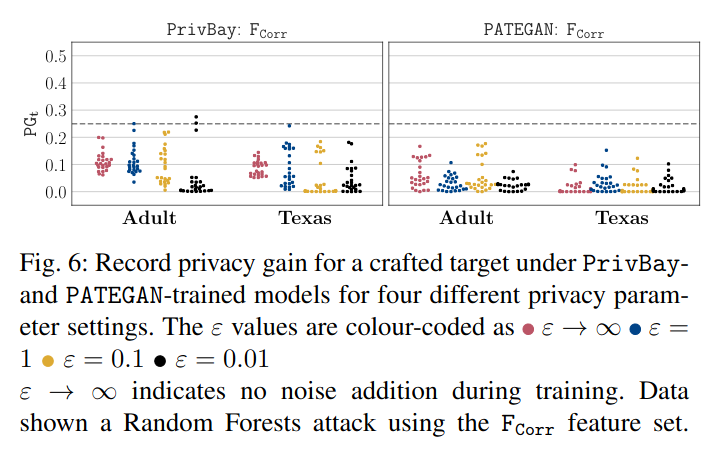
\includegraphics[scale=0.35]{images/fig6.png}
	\end{figure}
\end{frame}

\begin{frame}{High variance :: VIII.A, page {\small 12}}
	\vspace{1cm}
	\begin{figure}
	\centering
	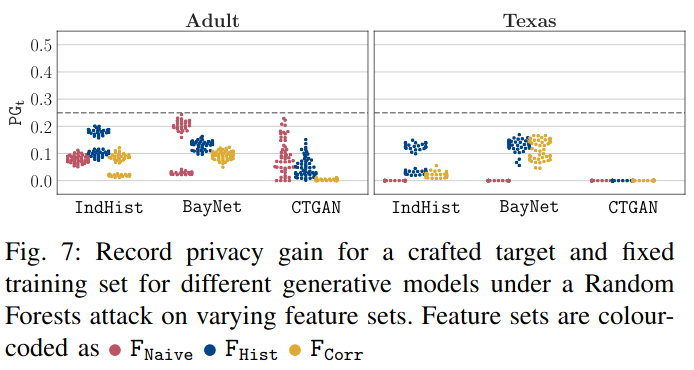
\includegraphics[scale=0.35]{images/fig7.png}
	\end{figure}
\end{frame}

\begin{frame}{High variance :: VIII.B, page {\small 13}}
	\vspace{1cm}
	\centertitle{Differential privacy}
	\begin{figure}
	\centering
	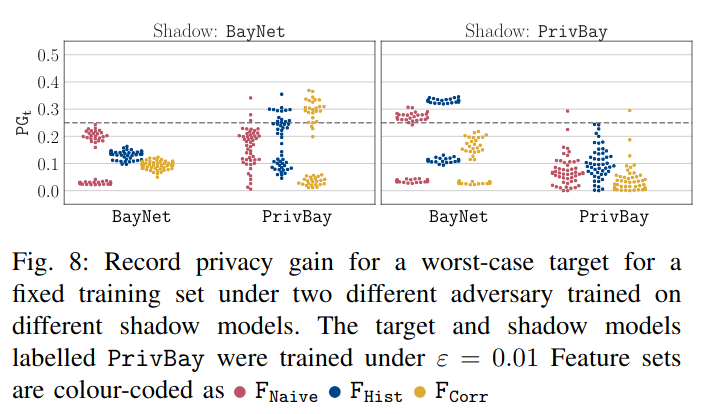
\includegraphics[scale=0.35]{images/fig8.png}
	\end{figure}
\end{frame}

\section{Conclusion}

\begin{frame}{Key takeaways :: IX}
	\begin{figure}
	\centering
	\begin{tikzpicture}
		\node[scale=0.33,draw=black,thick] (A) {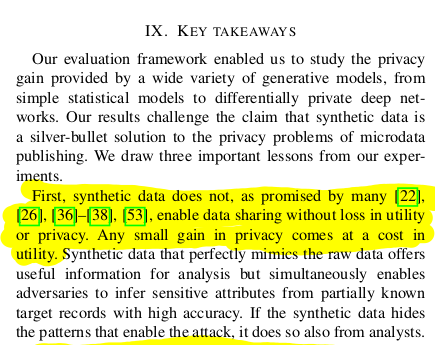
\includegraphics{images/takeaways1.png}};
		\node[scale=0.33,right=of A,draw=black,thick] (B) {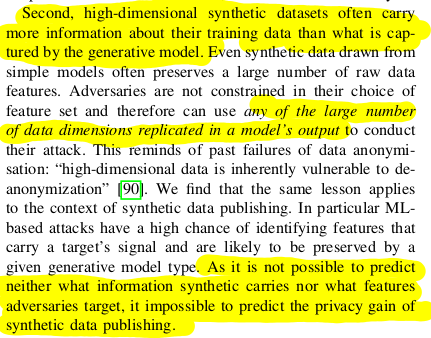
\includegraphics{images/takeaways2.png}};
		\node[yshift=-4cm,scale=0.33,draw=black,thick] at ($(A)!0.5!(B)$) (C) {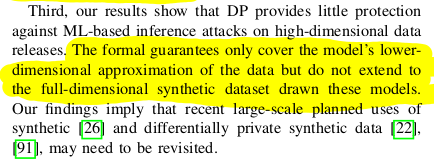
\includegraphics{images/takeaways3.png}};
	\end{tikzpicture}
	\end{figure}
\end{frame}

\begin{frame}{Potential research ideas}
	\vspace{1cm}
    \large{\begin{itemize}
        	\setlength\itemsep{3em}
        	\item<1-> Do these results translate to \hlcyan{synthetic graph data}?
        	\item<2-> Do these results have implications for the differential privacy policies used by the \hlorangeu{US 2020 census}?
        	\item<3-> Would \hlblue{public social media data} act as a training set for deanonymising public \hlblue{synthetic} datasets?
        \end{itemize}}
\end{frame}

\begin{frame}{References}
	\centering
	{\footnotesize
		\bibliographystyle{alpha}
		\bibliography{local}
	}
\end{frame}


\end{document}
